\chapter{Química ambiental y toxicología}\label{ch:b3:environmental-toxicology}

Cada final de verano, los satélites fotografían remolinos verdes que se extienden sobre grandes
lagos: proliferaciones de algas alimentadas por el fosfato y el nitrato que escurren de los campos y
salen de las ciudades. Cuando las algas mueren y se hunden, su descomposición consume el oxígeno de las
aguas profundas, y los peces mueren. La química explica cada eslabón de esa cadena, y de
muchas otras: por qué unos gases calientan el planeta y otros no, por qué la lluvia es
ácida incluso en un aire limpio, adónde va a parar un plaguicida una vez pulverizado, y qué
cantidad de una sustancia hace falta para causar daño. Este capítulo aplica los equilibrios,
la cinética y la espectroscopia a la atmósfera, las aguas naturales y los suelos, sigue a los
contaminantes entre ellos y termina con las cifras sobre las que se construyen las evaluaciones
de riesgos.

\begin{recall}
El volumen del primer año trató los equilibrios ácido--base, de precipitación y de complejación,
los diagramas potencial--pH, los coeficientes de reparto, los tiempos de semirreacción, el peligro,
el riesgo y el sistema SGA; el volumen escolar, los gases de efecto invernadero; el volumen del segundo año,
la ley de Henry, la fuerza iónica, la estadística, la espectrometría de masas y la espectrometría
atómica. El \cref{ch:b3:photochemistry} trató la fotoquímica atmosférica;
los \cref{ch:b3:group-theory-applied} y \cref{ch:b3:rovibrational-spectroscopy},
la actividad en el infrarrojo, y el \cref{ch:b3:surfaces-catalysis}, la \omterm{def:b3:surfaces-catalysis:adsorption}{adsorción}.
\end{recall}

\begin{omfigure}
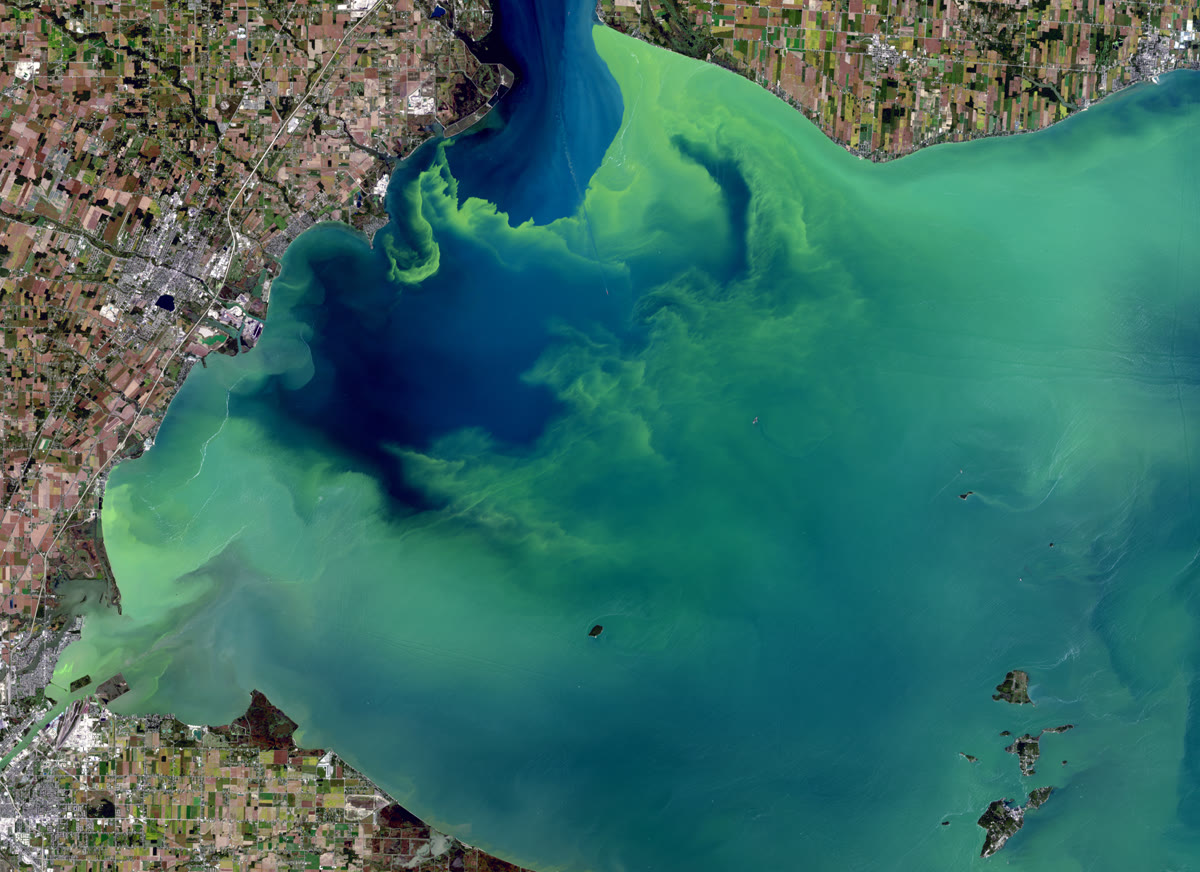
\includegraphics[width=0.62\linewidth]{images/book4/algal-bloom.jpg}

{\small Una proliferación de algas en un gran lago, vista por un satélite de observación de la Tierra a
finales de septiembre: los remolinos verdes son densas poblaciones de algas microscópicas
alimentadas por los nutrientes de las tierras de cultivo circundantes. Imagen: USGS y NASA, dominio público.}
\end{omfigure}

\section{La atmósfera}

\begin{definition}[Gases de efecto invernadero]\label{def:b3:environmental-toxicology:greenhouse}
Un \emph{gas de efecto invernadero}\index{gas de efecto invernadero} absorbe y emite radiación
infrarroja en las longitudes de onda de la radiación que emite la superficie terrestre, y
así calienta la baja atmósfera. El \emph{potencial de calentamiento
global}\index{potencial de calentamiento global} (PCG) de un gas en un horizonte temporal,
normalmente de 100 años, es la energía que retiene tras la emisión de un kilogramo,
relativa a la de un kilogramo de dióxido de carbono.
\end{definition}

Una molécula solo absorbe la radiación infrarroja mediante vibraciones que cambian su
momento dipolar (\cref{ch:b3:group-theory-applied}). El dinitrógeno y el dioxígeno,
diatómicas homonucleares, no tienen ninguna vibración así y son transparentes; el argón no tiene
ninguna vibración. El dióxido de carbono, lineal y apolar, tiene un modo de flexión activo en el
infrarrojo hacia \qty{15}{\micro\metre}, en plena emisión de la Tierra; el agua, el metano
y el óxido nitroso absorben a muchas longitudes de onda.

% ledger: atm:CO2.2025, atm:CH4.2025, atm:N2O.2025, gwp:CH4.fossil, gwp:CH4.nonfossil, gwp:N2O, life:CH4, life:N2O
En 2025, las fracciones molares medias mundiales eran de \qty{425.6}{ppm} de dióxido de carbono, \qty{1936}{ppb} de
metano y \qty{338.9}{ppb} de óxido nitroso. El metano, eliminado por los radicales hidroxilo con un
tiempo de vida de unos 12 años, tiene un PCG-100 de 27 a 30; el óxido nitroso, destruido solo en
la estratosfera con un tiempo de vida de unos 109 años, de 273. El dióxido de carbono no tiene un
tiempo de vida único: una parte de una emisión permanece en el aire durante siglos.

\begin{definition}[Contaminantes del aire]\label{def:b3:environmental-toxicology:pollutants}
Las \emph{partículas en suspensión}\index{particulas en suspension@partículas en suspensión} son las partículas sólidas y líquidas
suspendidas en el aire, clasificadas por su diámetro aerodinámico (las partículas finas,
de menos de \qty{2.5}{\micro\metre}, llegan hasta el fondo de los pulmones). La \emph{lluvia
ácida}\index{lluvia acida@lluvia ácida} es una lluvia más ácida que la lluvia limpia a causa de los ácidos sulfúrico y
nítrico formados a partir del dióxido de azufre y de los óxidos de nitrógeno.
\end{definition}

\begin{proposition}[pH de la lluvia limpia]\label{prop:b3:environmental-toxicology:rain-ph}
La lluvia en equilibrio con el dióxido de carbono del aire actual, y con nada
más, tiene un pH de alrededor de 5.6.
\end{proposition}

\begin{proof}
% ledger: henry:CO2, pka4:H2CO3.1, pkw4:25C, const:atm
La ley de Henry da $[\ce{CO2(aq)}] = K_Hp(\ce{CO2}) = \qty{3.4e-7}{mol.L^{-1}.Pa^{-1}} \times (425.6 \times 10^{-6} \times \qty{101325}{Pa}) = \qty{1.47e-5}{mol/L}$. El
balance de carga es $[\ce{H+}] = [\ce{HCO3-}] + 2[\ce{CO3^2-}] + [\ce{OH-}] \approx K_{a1}[\ce{CO2(aq)}]/[\ce{H+}] + K_w/[\ce{H+}]$, luego
$[\ce{H+}]^2 = K_{a1}[\ce{CO2(aq)}] + K_w = 10^{-6.35} \times \num{1.47e-5} + 10^{-14} = \num{6.6e-12}$: $[\ce{H+}] = \qty{2.6e-6}{mol/L}$, pH 5.6.
\end{proof}

El dióxido de azufre de la combustión de combustibles azufrados y los óxidos de nitrógeno de las
combustiones a alta temperatura se oxidan en el aire, por los radicales hidroxilo y en las gotitas
de las nubes, a ácidos sulfúrico y nítrico, que llevan la lluvia a un pH de 4 o inferior.
Eliminar el azufre de los combustibles y los óxidos de nitrógeno de los gases de escape (convertidores
catalíticos, inyección de amoníaco en las centrales eléctricas) ha resuelto en gran medida el problema
allí donde se ha aplicado. El ozono cercano al suelo, formado cuando la luz solar actúa sobre los
óxidos de nitrógeno y los compuestos orgánicos volátiles (\cref{ch:b3:photochemistry}), y
las partículas finas siguen siendo los principales contaminantes del aire para la salud.

\section{Aguas naturales}

\begin{omfigure}
\begin{tikzpicture}
\begin{axis}[name=a, width=0.48\linewidth, height=5.4cm, xmin=4, xmax=13, ymin=0, ymax=1.02,
  axis lines=left, xlabel={pH}, ylabel={fracción del carbono disuelto},
  tick label style={font=\scriptsize}, label style={font=\small}]
\addplot[color=omDef, thick] table[x=pH, y=a0] {figdata/out/bachelor-3-carbonate-system.dat};
\addplot[color=omMeth, thick] table[x=pH, y=a1] {figdata/out/bachelor-3-carbonate-system.dat};
\addplot[color=omThm, thick] table[x=pH, y=a2] {figdata/out/bachelor-3-carbonate-system.dat};
\node[font=\scriptsize, omDef] at (axis cs:4.9,0.85) {$\ce{CO2(aq)}$};
\node[font=\scriptsize, omMeth] at (axis cs:8.3,0.88) {$\ce{HCO3-}$};
\node[font=\scriptsize, omThm] at (axis cs:12.1,0.85) {$\ce{CO3^2-}$};
\draw[black!30, dashed] (axis cs:6.35,0) -- (axis cs:6.35,0.5) (axis cs:10.33,0) -- (axis cs:10.33,0.5);
\end{axis}
\begin{axis}[at={(a.east)}, anchor=west, xshift=1.4cm, width=0.48\linewidth, height=5.4cm,
  xmin=0, xmax=2000, ymin=5.2, ymax=6.2, axis lines=left,
  xlabel={$\ce{CO2}$ en el aire / ppm}, ylabel={pH de la lluvia},
  tick label style={font=\scriptsize}, label style={font=\small},
  scaled x ticks=false, xticklabel style={/pgf/number format/1000 sep={}}]
\addplot[color=omDef, thick] table[x=ppm, y=pH] {figdata/out/bachelor-3-carbonate-system-b.dat};
\draw[black!35, dashed] (axis cs:425.6,5.2) -- (axis cs:425.6,5.59);
\node[font=\scriptsize, anchor=west] at (axis cs:470,5.63) {hoy: 5.6};
\end{axis}
\end{tikzpicture}

{\small Izquierda: distribución del carbono inorgánico disuelto entre sus tres formas
en función del pH a \qty{25}{\celsius}, con cruces en $\mathrm pK_{a1} = 6.35$ y $\mathrm pK_{a2} = 10.33$. Derecha: pH de la lluvia en
equilibrio solo con el dióxido de carbono, en función de su fracción molar en el aire.}
\end{omfigure}

\begin{proposition}[Fracciones de carbonato]\label{prop:b3:environmental-toxicology:carbonate-fractions}
Siendo $C_T$ el carbono inorgánico disuelto total,
$[\ce{CO2(aq)}] = C_Th^2/D$, $[\ce{HCO3-}] = C_TK_{a1}h/D$, $[\ce{CO3^2-}] = C_TK_{a1}K_{a2}/D$, donde $h = [\ce{H+}]$ y $D = h^2 + K_{a1}h + K_{a1}K_{a2}$.
\end{proposition}

\begin{proof}
A partir de las dos constantes de acidez,
\[
  [\ce{HCO3-}] = \frac{K_{a1}[\ce{CO2(aq)}]}{h}, \qquad [\ce{CO3^2-}] = \frac{K_{a2}[\ce{HCO3-}]}{h} = \frac{K_{a1}K_{a2}[\ce{CO2(aq)}]}{h^2}.
\]
Su suma es $C_T = [\ce{CO2(aq)}]\,D/h^2$; dividiendo cada forma por $C_T$ se obtienen las fracciones.
\end{proof}

\begin{definition}[Alcalinidad]\label{def:b3:environmental-toxicology:alkalinity}
La \emph{alcalinidad}\index{alcalinidad} de un agua es su capacidad para neutralizar
un ácido fuerte, medida por valoración hasta el punto final del ácido carbónico (pH de alrededor
de 4.5) y expresada en moles de $\ce{H+}$ por litro.
\end{definition}

\begin{proposition}[Alcalinidad carbonatada]\label{prop:b3:environmental-toxicology:alkalinity}
En un agua cuyas bases son especies carbonatadas e hidróxido,
$\mathrm{Alc} = [\ce{HCO3-}] + 2[\ce{CO3^2-}] + [\ce{OH-}] - [\ce{H+}]$; es igual al exceso de las cargas de los cationes de bases fuertes
sobre las de los aniones de ácidos fuertes, y no cambia cuando el dióxido de carbono
se intercambia con el aire.
\end{proposition}

\begin{proof}
La valoración hasta el punto final del ácido carbónico convierte cada $\ce{HCO3-}$ en $\ce{CO2}$ (un $\ce{H+}$ cada uno),
cada $\ce{CO3^2-}$ en $\ce{CO2}$ (dos) y cada $\ce{OH-}$ en agua (uno), mientras que el $\ce{H+}$ libre ya presente
cuenta en contra: la suma enunciada. El balance de carga del agua, con
$\ce{Na+}$, $\ce{Ca^2+}$\dots{} y $\ce{Cl-}$, $\ce{SO4^2-}$\dots, se reordena en la misma suma, igual a $\sum z_i c_i$(cationes) $-$ $\sum z_jc_j$(aniones)
de los electrolitos fuertes. Añadir o quitar $\ce{CO2}$ no cambia ninguno de esos iones.
\end{proof}

\begin{definition}[Acidificación de los océanos]\label{def:b3:environmental-toxicology:acidification}
La \emph{acidificación de los océanos}\index{acidificacion de los oceanos@acidificación de los océanos} es la disminución del
pH del agua de mar a medida que absorbe dióxido de carbono del aire. El \emph{estado de
saturación}\index{estado de saturacion@estado de saturación} de un mineral carbonatado es
$\Omega = [\ce{Ca^2+}][\ce{CO3^2-}]/K_{sp}$: por encima de 1, el mineral puede formarse; por debajo de 1, tiende a disolverse.
\end{definition}

El dióxido de carbono disuelto convierte los iones carbonato en hidrogenocarbonato, $\ce{CO2 + CO3^2- + H2O -> 2HCO3-}$,
lo que rebaja el pH y $\Omega$: las conchas y los esqueletos de coral se vuelven más difíciles de construir. (En
el agua de mar, las constantes son constantes aparentes, medidas en el medio salino, y
difieren de los valores del agua dulce de este capítulo.)

\begin{definition}[Dureza del agua]\label{def:b3:environmental-toxicology:hardness}
La \emph{dureza}\index{dureza del agua} de un agua es su concentración total
de iones calcio y magnesio, expresada a menudo como la masa de carbonato de calcio
que contendría el mismo número de moles, en mg/L.
\end{definition}

\begin{definition}[Demanda de oxígeno]\label{def:b3:environmental-toxicology:oxygen-demand}
La \emph{demanda bioquímica de oxígeno}\index{demanda bioquimica de oxigeno@demanda bioquímica de oxígeno} (DBO) de un
agua es la masa de dioxígeno consumida por litro por los microorganismos que oxidan su
materia orgánica en la oscuridad, durante un tiempo determinado (cinco días a \qty{20}{\celsius} para la $\mathrm{DBO_5}$). Su
\emph{demanda química de oxígeno}\index{demanda quimica de oxigeno@demanda química de oxígeno} (DQO) es la masa de
dioxígeno equivalente al dicromato consumido al oxidar químicamente su materia
orgánica.
\end{definition}

\begin{proposition}[Curva de la DBO]\label{prop:b3:environmental-toxicology:bod}
Si la materia orgánica biodegradable se consume según una cinética de primer orden con constante de
velocidad $k$, el oxígeno consumido al cabo de un tiempo $t$ es $\mathrm{DBO}_t = L_0(1 - \eu^{-kt})$, donde $L_0$ es la DBO última.
\end{proposition}

\begin{proof}
La demanda restante $L$ obedece a $\dd L/\dd t = -kL$, luego $L = L_0\eu^{-kt}$; el oxígeno consumido es lo que ha desaparecido,
$L_0 - L$.
\end{proof}

\begin{omfigure}
\begin{tikzpicture}
\begin{axis}[name=a, width=0.48\linewidth, height=5.2cm, xmin=0, xmax=30, ymin=0, ymax=270,
  axis lines=left, xlabel={tiempo / días}, ylabel={DBO / \unit{mg.L^{-1}}},
  tick label style={font=\scriptsize}, label style={font=\small}]
\addplot[color=omDef, thick] table[x=t, y=bod] {figdata/out/bachelor-3-bod.dat};
\draw[black!35, dashed] (axis cs:0,250) -- (axis cs:30,250);
\draw[black!35, dashed] (axis cs:5,0) -- (axis cs:5,170.8);
\node[font=\scriptsize, anchor=west] at (axis cs:5.6,140) {$\mathrm{DBO_5}$};
\node[font=\scriptsize, anchor=north east] at (axis cs:30,246) {$L_0$};
\end{axis}
\begin{axis}[at={(a.east)}, anchor=west, xshift=1.4cm, width=0.48\linewidth, height=5.2cm,
  xmin=0, xmax=15, ymin=0, ymax=10, axis lines=left,
  xlabel={tiempo aguas abajo / días}, ylabel={$\ce{O2}$ disuelto / \unit{mg.L^{-1}}},
  tick label style={font=\scriptsize}, label style={font=\small}]
\addplot[color=omThm, thick] table[x=t, y=O2] {figdata/out/bachelor-3-bod-b.dat};
\draw[black!35, dashed] (axis cs:0,9.1) -- (axis cs:15,9.1);
\node[font=\scriptsize, anchor=south east] at (axis cs:15,9.1) {saturación};
\node[font=\scriptsize, anchor=north] at (axis cs:2.4,6.3) {punto crítico};
\end{axis}
\end{tikzpicture}

{\small Izquierda: la DBO de un agua residual modelo, $L_0 = \qty{250}{mg/L}$ y $k = \qty{0.23}{d^{-1}}$: unas dos terceras partes de la
demanda se consumen en cinco días. Derecha: la curva de déficit de oxígeno de un río aguas abajo de un vertido
(modelo de Streeter--Phelps): al principio, la descomposición de la carga orgánica consume el oxígeno más deprisa
de lo que el aire lo repone, hasta que el déficit alcanza su máximo al cabo de unos 2.4 días.}
\end{omfigure}

\begin{method}[Determinar la DQO]\label{met:b3:environmental-toxicology:cod}
\begin{enumerate}
  \item Calentar a reflujo un volumen medido de muestra con un exceso conocido de dicromato
        de potasio en ácido sulfúrico, con sulfato de plata como catalizador y
        sulfato de mercurio(II) para fijar el cloruro.
  \item Valorar el dicromato restante con hierro(II) usando ferroína, y realizar un
        blanco con agua pura.
  \item El dicromato consumido, convertido en la masa equivalente de $\ce{O2}$ (un
        $\ce{Cr2O7^2-}$ toma seis electrones, como lo harían 1.5 $\ce{O2}$), dividido por el volumen de la muestra, es la
        DQO en mg/L.
\end{enumerate}
\end{method}

\begin{definition}[Eutrofización]\label{def:b3:environmental-toxicology:eutrophication}
La \emph{eutrofización}\index{eutrofizacion@eutrofización} es el enriquecimiento de una masa de agua
en nutrientes, sobre todo fósforo y nitrógeno, que conduce a un crecimiento excesivo de las
algas y las plantas, y después al agotamiento del oxígeno cuando se descomponen.
\end{definition}

\begin{omfigure}
\begin{tikzpicture}[font=\scriptsize, >=Stealth,
  box/.style={draw, rounded corners, align=center, fill=omMeth!10, inner sep=3pt, minimum height=8mm}]
  \node[box] (f) at (-3.4,1.2) {campos: abonos,\\ estiércol};
  \node[box] (t) at (-3.4,-0.4) {ciudades: aguas\\ residuales,\\ detergentes};
  \node[box] (a) at (0,2.1) {atmósfera:\\ deposición (N)};
  \node[box, fill=omDef!12, minimum width=3.2cm, minimum height=1.7cm] (l) at (0.6,0.4) {agua del lago:\\ crecen las algas};
  \node[box, fill=black!8] (s) at (0.6,-1.6) {sedimento: P almacenado,\\ liberado en anoxia};
  \node[box] (o) at (4.0,0.4) {efluente};
  \draw[->, thick] (f) -- node[above, sloped, pos=0.4] {arrastre} (l);
  \draw[->, thick] (t) -- node[below, sloped] {N, P} (l);
  \draw[->, thick] (a) -- (l);
  \draw[->, thick] (l) -- node[left] {algas muertas} (s);
  \draw[->, thick, dashed] (s.east) to[bend right=30] node[right] {P} (l.south east);
  \draw[->, thick] (l) -- (o);
\end{tikzpicture}

{\small Flujos de nutrientes hacia un lago y dentro de él. El fósforo, a menudo el nutriente
limitante en el agua dulce, se acumula en el sedimento y vuelve al agua
cuando el fondo pierde su oxígeno, lo que puede mantener las proliferaciones durante años después de
reducir los aportes.}
\end{omfigure}

Las algas absorben carbono, nitrógeno y fósforo en proporciones aproximadamente constantes;
el nutriente que escasea respecto de esas necesidades limita su crecimiento. En
la mayoría de los lagos es el fósforo, por lo que se eliminaron los fosfatos de los
detergentes y de las aguas residuales tratadas; en muchos mares costeros es el nitrógeno.

\begin{definition}[Especiación]\label{def:b3:environmental-toxicology:speciation}
La \emph{especiación química}\index{especiacion quimica@especiación química} de un elemento en una
muestra es la distribución de su cantidad entre sus formas químicas: estados de
oxidación, complejos, compuestos organometálicos, especies libres y unidas.
\end{definition}

La toxicidad depende de la especiación. El mercurio inorgánico liberado en el agua es
metilado por las bacterias de los sedimentos a metilmercurio, que atraviesa las membranas,
se une al azufre de las proteínas y se concentra a lo largo de las cadenas tróficas; el arsénico es mucho más
tóxico como arsenito, As(III), que como arseniato, As(V), y mucho menos en las formas orgánicas
presentes en el marisco. Una concentración total por sí sola dice poco.

\begin{method}[Especiación de un metal en un agua]\label{met:b3:environmental-toxicology:speciation}
\begin{enumerate}
  \item Enumerar los ligandos presentes (hidróxido, carbonato, cloruro, sulfato, materia
        orgánica) con sus concentraciones y el pH.
  \item Escribir las constantes de complejación y el balance de masa del metal, como en el
        volumen del primer año.
  \item Despejar el ion metálico libre y después cada complejo; representar las fracciones en función
        del pH o de la concentración de un ligando.
  \item Comparar la forma tóxica o biodisponible (a menudo el ion libre) con el total.
\end{enumerate}
\end{method}

\section{Suelos y sedimentos}

\begin{definition}[Sorción en los suelos]\label{def:b3:environmental-toxicology:soil}
La \emph{capacidad de intercambio catiónico}\index{capacidad de intercambio cationico@capacidad de intercambio catiónico} de un suelo es
la cantidad de cationes intercambiables que puede retener por unidad de masa, en las arcillas y la materia
orgánica. El \emph{coeficiente de distribución suelo--agua}\index{coeficiente de distribucion suelo--agua@coeficiente de distribución suelo--agua}
$K_d$ es la razón entre la concentración de una sustancia
sorbida en el suelo (por kilogramo) y su concentración en el agua intersticial (por
litro); el \emph{coeficiente de reparto en carbono orgánico}\index{coeficiente de reparto en carbono organico@coeficiente de reparto en carbono orgánico}
es $K_{oc} = K_d/f_{oc}$, donde $f_{oc}$ es la fracción másica de carbono orgánico.
\end{definition}

Los compuestos orgánicos neutros se sorben sobre todo en la materia orgánica del suelo, de modo que $K_{oc}$ varía
mucho menos de un suelo a otro que $K_d$. Un compuesto con una $K_d$ pequeña se desplaza con el agua
y puede llegar a las aguas subterráneas (lixiviación); uno con una $K_d$ grande permanece cerca de la superficie,
unido a partículas que la erosión puede arrastrar a los ríos y los lagos.

\section{Destino de los contaminantes}

\begin{definition}[Coeficiente de reparto octanol--agua]\label{def:b3:environmental-toxicology:kow}
El \emph{coeficiente de reparto octanol--agua}\index{coeficiente de reparto octanol--agua}
$K_{ow}$ de una sustancia es la razón entre sus concentraciones de equilibrio en el
octan-1-ol y en el agua; mide su afinidad por los tejidos grasos y la materia
orgánica.
\end{definition}

% ledger: logkow:DDT, logkow:benzene, logkow:atrazine, logkow:PCB153
El benceno tiene $\log K_{ow} = 2.13$; el herbicida atrazina, 2.61; un PCB hexaclorado, 6.67, y el
DDT, 6.91: los dos últimos se disuelven en la grasa decenas de millones de veces mejor que en el
agua.

\begin{definition}[Bioacumulación]\label{def:b3:environmental-toxicology:bio}
El \emph{factor de bioconcentración}\index{factor de bioconcentracion@factor de bioconcentración} (FBC) es la
razón entre la concentración en un organismo y la del agua que lo rodea en el estado
estacionario, con absorción solo a partir del agua. La \emph{bioacumulación}\index{bioacumulacion@bioacumulación}
es la acumulación en un organismo por todas las vías, alimentación incluida;
la \emph{biomagnificación}\index{biomagnificacion@biomagnificación} es el aumento de la
concentración de presa a depredador a lo largo de una cadena trófica.
\end{definition}

\begin{proposition}[FBC y $K_{ow}$]\label{prop:b3:environmental-toxicology:bcf-kow}
Para las sustancias orgánicas neutras que no se metabolizan, el $\log\mathrm{FBC}$ en los peces es
aproximadamente una función lineal del $\log K_{ow}$, con una pendiente próxima a 1, hasta un $\log K_{ow}$ cercano a 6;
por encima, la absorción se ralentiza y la relación se estabiliza (regresiones empíricas).
\admitted
\end{proposition}

\begin{definition}[Contaminantes orgánicos persistentes]\label{def:b3:environmental-toxicology:pop}
Un \emph{contaminante orgánico persistente}\index{contaminante organico persistente@contaminante orgánico persistente} es una
sustancia orgánica que resiste la degradación, se bioacumula, es tóxica y se
transporta lejos de sus fuentes, como el DDT, los PCB y las dioxinas.
\end{definition}

\begin{proposition}[Distribución de equilibrio entre compartimentos]\label{prop:b3:environmental-toxicology:level-one}
Una masa $M$ de una sustancia distribuida en el equilibrio (un modelo de ``nivel I'') entre el agua
(volumen $V_w$), el aire ($V_a$), los sólidos del sedimento ($m_s$) y los peces ($m_f$) tiene la concentración en el agua
$C_w = M/(V_w + K_{aw}V_a + K_{sw}m_s + K_{fw}m_f)$, donde las $K$ son los coeficientes de reparto respecto del
agua; la masa de cada compartimento es su término multiplicado por $C_w$.
\end{proposition}

\begin{proof}
En el equilibrio, $C_a = K_{aw}C_w$, $C_s = K_{sw}C_w$ (por kilogramo), $C_f = K_{fw}C_w$. El balance de masa es
$M = C_wV_w + C_aV_a + C_sm_s + C_fm_f = C_w(V_w + K_{aw}V_a + K_{sw}m_s + K_{fw}m_f)$; dividiendo se obtiene $C_w$.
\end{proof}

\begin{omfigure}
\begin{tikzpicture}[font=\scriptsize, >=Stealth,
  comp/.style={draw, rounded corners, align=center, minimum width=2.6cm, minimum height=1.0cm}]
  \node[comp, fill=omDef!8] (air) at (0,2.2) {aire\\ $C_a = K_{aw}C_w$};
  \node[comp, fill=omDef!25] (w) at (0,0.6) {agua\\ $C_w$};
  \node[comp, fill=black!10] (sed) at (0,-1.0) {sedimento\\ $C_s = K_{sw}C_w$};
  \node[comp, fill=omMeth!15] (fish) at (3.6,0.6) {peces\\ $C_f = K_{fw}C_w$};
  \node[comp, fill=omProp!15] (soil) at (-3.6,0.6) {suelo\\ $C_{\mathrm{suelo}} = K_dC_w$};
  \draw[<->, thick] (air) -- (w); \draw[<->, thick] (w) -- (sed);
  \draw[<->, thick] (w) -- (fish); \draw[<->, thick] (w) -- (soil);
\end{tikzpicture}

{\small Compartimentos de un modelo de equilibrio (de nivel I): cada compartimento está en
equilibrio con el agua, y su concentración la fija un coeficiente de reparto.
La sustancia se acumula allí donde es mayor el producto de la capacidad por el volumen (o la masa),
a menudo el sedimento o el suelo para un compuesto hidrófobo.}
\end{omfigure}

\section{Toxicología y reglamentación}

\begin{definition}[Dosis--respuesta]\label{def:b3:environmental-toxicology:dose}
Una \emph{relación dosis--respuesta}\index{relacion dosis--respuesta@relación dosis--respuesta} relaciona
la dosis de una sustancia con la magnitud o la frecuencia de un efecto. La \emph{dosis letal
media}\index{dosis letal media} $\mathrm{DL_{50}}$ mata a la mitad de una población de ensayo; la
\emph{concentración efectiva media}\index{concentracion efectiva media@concentración efectiva media} $\mathrm{CE_{50}}$
causa un efecto determinado en la mitad. El \emph{nivel sin efecto adverso
observado}\index{nivel sin efecto adverso observado} (NOAEL) es la dosis ensayada más alta
sin efecto adverso, y el \emph{nivel mínimo con efecto adverso
observado}\index{nivel minimo con efecto adverso observado@nivel mínimo con efecto adverso observado} (LOAEL), la dosis ensayada más baja
con efecto adverso.
\end{definition}

\begin{proposition}[Modelo log-logístico]\label{prop:b3:environmental-toxicology:dose-response}
En el modelo log-logístico $f(d) = 1/\bigl(1 + (D_{50}/d)^n\bigr)$, la respuesta vale la mitad en $d = D_{50}$, y $n$
mide la pendiente: la razón de dosis entre las respuestas del 10\,\% y del 90\,\% es $81^{1/n}$.
\end{proposition}

\begin{proof}
En $d = D_{50}$, $f = 1/2$. $f = 0.1$ exige $(D_{50}/d)^n = 9$, y $f = 0.9$ exige $(D_{50}/d)^n = 1/9$; la razón entre las dos dosis
es $(9 \times 9)^{1/n} = 81^{1/n}$.
\end{proof}

\begin{omfigure}
\begin{tikzpicture}
\begin{axis}[width=0.72\linewidth, height=5.4cm, xmode=log, xmin=3, xmax=3200, ymin=0, ymax=1.02,
  axis lines=left, xlabel={dosis / \unit{mg.kg^{-1}}}, ylabel={fracción que responde},
  tick label style={font=\scriptsize}, label style={font=\small}]
\addplot[color=omDef, thick] table[x=d, y=n2] {figdata/out/bachelor-3-dose-response.dat};
\addplot[color=omThm, thick] table[x=d, y=n6] {figdata/out/bachelor-3-dose-response.dat};
\addplot[only marks, mark=*, mark size=1.6pt, omThm] table[x=d, y=r] {figdata/out/bachelor-3-dose-response-b.dat};
\draw[black!35, dashed] (axis cs:200,0) -- (axis cs:200,0.5) -- (axis cs:3,0.5);
\node[font=\scriptsize, anchor=north west] at (axis cs:200,0.48) {$D_{50}$};
\node[font=\scriptsize, omThm, anchor=south east, inner sep=1pt] (noael) at (axis cs:60,0.09) {NOAEL};
\draw[omThm] (noael.south east) -- (axis cs:78,0.012);
\node[font=\scriptsize, omThm, anchor=west] at (axis cs:165,0.2) {LOAEL};
\node[font=\scriptsize, omDef, anchor=east] at (axis cs:60,0.25) {$n = 2$};
\node[font=\scriptsize, omThm, anchor=east] at (axis cs:185,0.8) {$n = 6$};
\end{axis}
\end{tikzpicture}

{\small Curvas dosis--respuesta log-logísticas con la misma dosis media (\qty{200}{mg/kg},
modelo) y dos pendientes. Los puntos son un estudio con cinco dosis para la curva
más pronunciada: con una respuesta del 5\,\% como criterio de efecto adverso, el NOAEL es de
\qty{80}{mg/kg} y el LOAEL de \qty{160}{mg/kg}; ambos dependen de las dosis elegidas.}
\end{omfigure}

\begin{definition}[Toxicidad aguda y crónica]\label{def:b3:environmental-toxicology:toxicity}
La \emph{toxicidad aguda}\index{toxicidad aguda} es el daño causado por una sola
exposición o por exposiciones en un corto intervalo de tiempo; la \emph{toxicidad crónica}\index{toxicidad cronica@toxicidad crónica},
el causado por una exposición repetida o continua durante una parte importante de la vida.
\end{definition}

% ledger: ld50:NaCl, ld50:caffeine, ld50:nicotine
La toxicidad es una cuestión de dosis: la $\mathrm{DL_{50}}$ oral en la rata es de unos \qty{3000}{mg/kg} para el cloruro de sodio,
\qty{192}{mg/kg} para la cafeína y \qty{188}{mg/kg} para la nicotina en el mismo tipo de registro. Para la mayoría de los efectos existe una
dosis umbral por debajo de la cual el organismo se las arregla; para los cancerígenos genotóxicos
no se supone ninguna, y la exposición se mantiene tan baja como sea razonablemente posible.

\begin{definition}[Ecotoxicología]\label{def:b3:environmental-toxicology:ecotoxicology}
La \emph{ecotoxicología}\index{ecotoxicologia@ecotoxicología} estudia los efectos de las sustancias sobre
los organismos en los ecosistemas. La \emph{concentración prevista sin
efecto}\index{concentracion prevista sin efecto@concentración prevista sin efecto} (PNEC) es la menor concentración
con efecto o sin efecto obtenida en ensayos con especies representativas,
dividida por un factor de evaluación que cubre la incertidumbre; la
\emph{concentración ambiental prevista}\index{concentracion ambiental prevista@concentración ambiental prevista}
(PEC) es la concentración esperada a partir de los usos y del destino de la
sustancia; el \emph{cociente de riesgo}\index{cociente de riesgo} es PEC/PNEC.
\end{definition}

\begin{proposition}[Cociente de riesgo]\label{prop:b3:environmental-toxicology:risk-quotient}
Un \omterm{def:b3:environmental-toxicology:ecotoxicology}{cociente de riesgo} inferior a 1 indica que no hay motivo de preocupación para el compartimento evaluado; superior a
1, un riesgo que exige datos más precisos o medidas para reducir la exposición.
\end{proposition}

\begin{proof}[Por definición]
La PNEC se fija, mediante su factor de evaluación, por debajo de las concentraciones a las que
se observaron efectos; una concentración esperada inferior a ella no debería, por tanto,
causar efectos, y una superior, sí.
\end{proof}

\begin{method}[Una evaluación del riesgo ambiental]\label{met:b3:environmental-toxicology:risk}
\begin{enumerate}
  \item Peligro: reunir los datos de toxicidad para algas, invertebrados y peces ($\mathrm{CE_{50}}$
        aguda, NOEC crónica); tomar el más bajo; dividirlo por el factor de evaluación (mayor cuando
        solo existen datos agudos) para obtener la PNEC.
  \item Exposición: a partir de las cantidades usadas y del destino (reparto, degradación),
        calcular la PEC en cada compartimento, o medirla.
  \item Riesgo: calcular PEC/PNEC; si es superior a 1, afinar los datos o reducir la
        exposición, y repetir.
\end{enumerate}
\end{method}

\begin{definition}[Límite de exposición profesional]\label{def:b3:environmental-toxicology:oel}
Un \emph{límite de exposición profesional}\index{limite de exposicion profesional@límite de exposición profesional} es la
concentración de una sustancia en el aire de un lugar de trabajo que los trabajadores pueden respirar,
promediada sobre una jornada de trabajo (o sobre 15 minutos para los límites de corta duración), sin
efectos adversos esperados.
\end{definition}

Las sustancias químicas nuevas comercializadas en cantidad deben registrarse con un
expediente de sus propiedades, sus peligros y sus usos; las más peligrosas pueden
restringirse o permitirse solo para usos autorizados.

\begin{inthelab}[Medir la $\mathrm{DBO_5}$]
Se diluye una muestra con agua de dilución aireada que contiene nutrientes y un
inóculo bacteriano, de modo que se consuma una buena parte, pero no todo, del oxígeno. Se llenan
hasta el borde dos frascos con tapón: el oxígeno disuelto de uno se mide
enseguida con un electrodo de oxígeno, y el del otro, al cabo de cinco días en la oscuridad a
\qty{20}{\celsius}. La diferencia, multiplicada por el factor de dilución y corregida por el inóculo, es la
$\mathrm{DBO_5}$.
\end{inthelab}

\begin{safety}{\ghs[0.62cm]{GHS03}\ghs[0.62cm]{GHS05}\ghs[0.62cm]{GHS06}\ghs[0.62cm]{GHS08}\ghs[0.62cm]{GHS09}}
% ledger: ghs:K2Cr2O7, ghs4:HgSO4
Los reactivos de la DQO: el dicromato de potasio es comburente, puede provocar cáncer y
defectos genéticos, es corrosivo y sensibilizante; el sulfato de mercurio(II) es mortal en caso de
ingestión, inhalación o contacto con la piel, y muy tóxico para los organismos acuáticos. Ambos se
usan en tubos sellados, y los tubos usados van a los residuos peligrosos.
\end{safety}

\begin{history}[Un libro y una bahía]
En 1962, \textit{Primavera silenciosa}, de Rachel Carson, describió el declive de las aves envenenadas por el
DDT y otros plaguicidas concentrados a lo largo de las cadenas tróficas, e impulsó la reglamentación
ambiental moderna. Unos años antes, en 1956, se reconoció una enfermedad del sistema
nervioso entre los habitantes de la bahía de Minamata: una planta química había
vertido metilmercurio, formado a partir de su catalizador de mercurio, que se acumuló
en los peces que comían los habitantes.
\end{history}

\section{Ejercicios}

\begin{exercise}[$\star$]\label{exo:b3:environmental-toxicology:1}
¿Por qué el $\ce{N2}$, el $\ce{O2}$ y el Ar no absorben en el infrarrojo, y qué vibración del $\ce{CO2}$ hace de él un
\omterm{def:b3:environmental-toxicology:greenhouse}{gas de efecto invernadero}?
\end{exercise}

\begin{exercise}[$\star$]\label{exo:b3:environmental-toxicology:2}
¿En qué factor cambia $[\ce{H+}]$ cuando el pH del agua de mar disminuye en 0.1?
\end{exercise}

\begin{exercise}[$\star$]\label{exo:b3:environmental-toxicology:3}
Un agua contiene \qty{2.0}{mmol/L} de $\ce{Ca^2+}$ y \qty{0.50}{mmol/L} de $\ce{Mg^2+}$. Dese su \omterm{def:b3:environmental-toxicology:hardness}{dureza} en mg de $\ce{CaCO3}$ por litro.
\end{exercise}

\begin{exercise}[$\star$]\label{exo:b3:environmental-toxicology:4}
Las algas absorben C, N y P en la razón molar $106 : 16 : 1$ (datos del ejercicio). Un agua de lago
tiene \qty{0.60}{mg/L} de nitrógeno de nitrato y \qty{0.010}{mg/L} de fósforo de fosfato. ¿Qué nutriente limita
el crecimiento?
\end{exercise}

\begin{exercise}[$\star\star$]\label{exo:b3:environmental-toxicology:5}
Se mide una $\mathrm{DBO_5}$ de \qty{170}{mg/L} en un agua residual con $k = \qty{0.23}{d^{-1}}$. Estímese su DBO última.
\end{exercise}

\begin{exercise}[$\star\star$]\label{exo:b3:environmental-toxicology:6}
Una muestra de agua de \qty{100.0}{mL} necesita \qty{4.40}{mL} de ácido clorhídrico \qty{0.0200}{mol/L} para alcanzar pH 4.5. Calcúlese su
\omterm{def:b3:environmental-toxicology:alkalinity}{alcalinidad} y, suponiendo que todo es hidrogenocarbonato, su concentración en mg/L.
\end{exercise}

\begin{exercise}[$\star\star$]\label{exo:b3:environmental-toxicology:7}
Un suelo tiene $f_{oc} = 0.020$; un plaguicida tiene $K_{oc} = \qty{300}{L/kg}$ (datos del ejercicio). Calcúlense $K_d$ y la
fracción del plaguicida sorbida en un suelo con \qty{1.5}{kg} de sólido por \qty{0.30}{L} de agua intersticial.
\end{exercise}

\begin{exercise}[$\star\star$]\label{exo:b3:environmental-toxicology:8}
Con $\log\mathrm{FBC} = 0.85\log K_{ow} - 0.70$ (una regresión empírica; datos del ejercicio), estímese el FBC del
benceno y el de un PCB hexaclorado, y coméntese.
\end{exercise}

\begin{exercise}[$\star\star$]\label{exo:b3:environmental-toxicology:9}
Exprésese la $\mathrm{DL_{50}}$ oral en la rata de la cafeína como una masa para un adulto de \qty{70}{kg} y como tazas de café de
\qty{90}{mg} cada una (un escalado ingenuo; datos del ejercicio). ¿Por qué un escalado así solo es orientativo?
\end{exercise}

\begin{exercise}[$\star\star\star$]\label{exo:b3:environmental-toxicology:10}
Una sustancia tiene una $\mathrm{CE_{50}}$ a 48 horas de \qty{0.50}{mg/L} para las pulgas de agua, una $\mathrm{CE_{50}}$ a 72 horas de \qty{1.2}{mg/L} para las algas
y una $\mathrm{CL_{50}}$ a 96 horas de \qty{2.0}{mg/L} para los peces, todas agudas, y se aplica un factor de evaluación de 1000
(datos del ejercicio). Calcúlense la PNEC y el \omterm{def:b3:environmental-toxicology:ecotoxicology}{cociente de riesgo} para una PEC de \qty{0.20}{\micro g/L}.
\end{exercise}

\begin{exercise}[$\star\star\star$]\label{exo:b3:environmental-toxicology:11}
Un ave piscívora come peces con \qty{0.30}{mg/kg} de un contaminante persistente; los peces comen
plancton con \qty{0.015}{mg/kg}; el agua contiene \qty{2.0}{ng/L}. Calcúlense los \omterm{def:b3:environmental-toxicology:bio}{factores de bioconcentración} y de
\omterm{def:b3:environmental-toxicology:bio}{biomagnificación} a lo largo de la cadena si la grasa del ave contiene \qty{6.0}{mg/kg} (datos del
ejercicio).
\end{exercise}

\begin{exercise}[$\star\star\star$]\label{exo:b3:environmental-toxicology:12}
Una central eléctrica emite \qty{1000}{t} de $\ce{SO2}$ al año. Calcúlese la masa de ácido sulfúrico que puede formar,
y el volumen de lluvia que llevaría a pH 4.0 si cayera todo con la lluvia (despréciense los demás
ácidos y bases).
\end{exercise}

\section{Problema: un plaguicida en un lago}

\begin{problem}[{Problema de fin de semana --- un plaguicida en un lago: su reparto entre el
sedimento y los peces, un balance de masa de equilibrio, su degradación a lo largo de un año
y el cociente de riesgo para los organismos del lago}]
\label{pb:b3:environmental-toxicology:1}
Datos del problema. Un lago contiene $\qty{1.0e9}{L}$ de agua bajo $\qty{1.0e12}{L}$ de aire (la capa de mezcla que lo cubre),
con $\qty{1.0e8}{kg}$ de sólidos de sedimento activo ($f_{oc} = 0.040$) y $\qty{1.0e4}{kg}$ de peces (fracción lipídica de 0.048).
Un plaguicida tiene $\log K_{ow} = 4.0$, un coeficiente de reparto aire--agua $K_{aw} = \num{1.0e-4}$ y $K_{oc} = 0.41\,K_{ow}$;
$K_{fw}$ = fracción lipídica $\times K_{ow}$. Llegan al lago 100 kg de él. Su tiempo de semirreacción en el lago es de 60 días.
El ensayo crónico más sensible da una NOEC de \qty{50}{\micro g/L}, con un factor de evaluación de 10;
los peces destinados al consumo humano no deben superar \qty{1.0}{mg/kg}.

\medskip\noindent\textbf{Parte I --- Coeficientes de reparto.}
\begin{enumerate}
  \item ¿Qué indica $\log K_{ow} = 4.0$ sobre el plaguicida?
  \item Calcúlense $K_{oc}$ y el coeficiente sedimento--agua $K_{sw}$.
  \item Calcúlese el coeficiente pez--agua $K_{fw}$.
  \item ¿Es volátil el plaguicida a partir del agua? Úsese $K_{aw}$.
  \item ¿Por qué rige su sorción el carbono orgánico, y no la materia mineral?
  \item ¿Qué compartimento cabe esperar que contenga la mayor parte?
\end{enumerate}

\medskip\noindent\textbf{Parte II --- Balance de masa de equilibrio.}
\begin{enumerate}[resume]
  \item Calcúlense los términos de capacidad $V_w$, $K_{aw}V_a$, $K_{sw}m_s$ y $K_{fw}m_f$.
  \item Calcúlese la concentración en el agua.
  \item Calcúlese la masa de cada compartimento.
  \item Calcúlense las concentraciones en el aire, el sedimento y los peces.
  \item ¿Qué hipótesis del modelo es la menos realista?
  \item ¿Cómo cambiaría la degradación el panorama (modelos de niveles II y III)?
\end{enumerate}

\medskip\noindent\textbf{Parte III --- Degradación.}
\begin{enumerate}[resume]
  \item Calcúlese la constante de velocidad de primer orden.
  \item Calcúlese la fracción que queda al cabo de un año.
  \item Calcúlese la concentración en el agua al cabo de un año.
  \item ¿Por qué el sedimento puede retener el plaguicida más tiempo del que sugiere el tiempo de semirreacción?
  \item ¿Qué hace persistente a un plaguicida?
\end{enumerate}

\medskip\noindent\textbf{Parte IV --- Riesgo.}
\begin{enumerate}[resume]
  \item Calcúlese la PNEC.
  \item Tómese como PEC la concentración inicial en el agua: calcúlese el \omterm{def:b3:environmental-toxicology:ecotoxicology}{cociente de riesgo}.
  \item Extráiganse conclusiones para los organismos del lago.
  \item Compárese la concentración en los peces con el umbral de consumo.
  \item ¿Qué se mediría a continuación, y dónde?
  \item ¿Qué medidas rebajarían la PEC?
  \item ¿Por qué importa tanto el factor de evaluación?
  \item Enúnciese el resultado: el \omterm{def:b3:environmental-toxicology:ecotoxicology}{cociente de riesgo} PEC/PNEC.
\end{enumerate}
\end{problem}
